%!TeX root = thesis-main.tex
%%%%%%%    AC     %%%%%%%
\newcommand{\export}{export}
\newcommand{\round}{round}
%%%%%%%    RL     %%%%%%%

%% Utils
\newcommand{\decision}[1]{{\color{red} #1}}
\newcommand{\mtext}[1]{\text{\texttt{#1}}}
%\newcommand{\revision}[1]{{#1}}
\newenvironment{iequation}{\(}{\). }
\def\tablename{Table}
\sloppypar
%% Acronyms

\newcommand{\scafiinline}[1]{\lstinline[language=scafi]$#1$}
%\end{lstlisting}

%\chapter{Addressing Collective Computations Efficiency: Towards a Platform-level Reinforcement Learning Approach}

\chapter[Platform: Addressing Collective Computations Efficiency---a Platform-level Reinforcement Learning Approach]{Platform: Addressing Collective Computations Efficiency---a Platform-level Reinforcement Learning Approach}\label{chap:rl:schedulers}%\mtcaddchapter
\minitoc% Creating an actual minitoc
%%!TeX root = thesis-main.tex
\acrodef{acml}[AC+ML]{aggregate computing + machine learning}
\acrodef{ml}[ML]{machine learning}
\acrodef{hql}[HQL]{Hysteretic Q-Learning}
\acrodef{qos}[QoS]{Quality of Service}
\acrodef{cps}[CPS]{Cyber-Physical System}
\acrodef{ict}[ICT]{Information-Communication Technology}
\acrodef{cmarl}[CMARL]{cooperative many-agent reinforcement learning}
\acrodef{dsl}[DSL]{Domain Specific Language}
\acrodef{ac}[AC]{aggregate computing}
\acrodef{AC}[AC]{aggregate computing}
\acrodef{dql}[DQL]{Distributed Q-Learning}
\acrodef{fc}[FC]{field calculus}
\acrodef{qos}[QoS]{Quality of Service}
\acrodef{cps}[CPS]{Cyber-Physical System}
\acrodef{DecPOMDP}[DecPOMDP]{decentralized partially observable Markov decision processes}
\acrodef{RL}[RL]{reinforcement learning}
\acrodef{MARL}[MARL]{multi-agent reinforcement learning}
\acrodef{MAARL}[ManyRL]{many-agent reinforcement learning}
\acrodef{MLP}[MLP]{multi-layer perceptron}
\acrodef{GNN}[GNN]{graph neural network}
\acrodef{CNN}[CNN]{convolutional neural network}
\acrodef{CTDE}[CTDE]{centralized training and decentralized execution}
\acrodef{ctde}[CTDE]{centralized training and decentralized execution}
\acrodef{DQN}[DQN]{Deep Q-Learning}
\acrodef{FIRL}[FIRL]{Field-Informed Reinforcement Learning}
\acrodef{api}[API]{Application Program Interface}
\acrodef{CAS}[CAS]{Collective Adaptive System}
\acrodef{cpsw}[CPSW]{Cyber-Physical Swarm}
\acrodef{iot}[IoT]{Internet of Things}
\acrodef{it}[IT]{Information Technology}
\acrodef{ci}[CI]{Collective Intelligence}
\acrodef{lidar}[LIDAR]{Laser Imaging Detection And Ranging}
\acrodef{le}[LE]{leader election}
\acrodef{frp}[FRP]{functional reactive programming}
\acrodef{mle}[MLE]{multi-leader election}
\acrodef{langname}[FRASP]{Functional Reactive Approach to Self-organization Programming}
\acrodef{algo}[Bounded Election]{Bounded Election}
\acrodef{rl}[RL]{reinforcement learning}
\acrodef{cct}[CCT]{concurrent collective task}
\acrodef{dd}[DD]{decentralization domain}
%\acrodef{dbms}[DBMS]{database management system}
\acrodef{dcp}[DCP]{distributed computational process}
\acrodefplural{dcp}[DCPs]{distributed computational processes}
\acrodef{RL}[RL]{reinforcement learning}
%\acrodef{ict}[ICT]{information and communication technology}
%\acrodef{it}[IT]{information technology}
%\acrodef{oca}[OCA]{overlapping collective activity}
\acrodef{mape}[MAPE]{monitor--analyse--plan--execute}
\acrodef{scr}[SCR]{self-organizing coordination regions}
\acrodef{wsn}[WSN]{wireless sensor network}

\acrodef{cas}[CAS]{Collective Adaptive System}
\acrodef{marl}[MARL]{multi-agent reinforcement learning}
\acrodef{mdp}[MDP]{Markov Decision Process}
\acrodef{MDP}[MDP]{Markov Decision Process}
\acrodef{qos}[QoS]{Quality of Service}
%\lstset{language=scafi}

An aggregate program is typically deployed
 to a network of neighbour-interacting devices
 that will execute it 
 through asynchronous sense-compute-act \emph{rounds}.
%
%In particular, \ac{AC} follows a pragmatic methodology in which the collective behaviours could be reused in different applications since it is decoupled from the underline IT architecture. 
%
The idea is that collective behaviour 
 has to emerge by repeated evaluation of the aggregate program,
 which describes computations and communications
 needed to steer the system (and its self-organization)
 towards globally coherent goals.
%
An aggregate program deals both with \emph{functional} aspects (i.e, how the overall ensemble should behave) 
 and \emph{non-functional aspects} (e.g., resilience as well as time, memory, and message complexity).
%
In part, non-functional aspects 
 can also be addressed by system designers
 at the middleware level.
%while the burden of managing non-functional aspects (e.g., energy consumption, bandwidth consumption, convergence time, etc.) is left to the \emph{execution platform}.
%
An \ac{AC} execution platform (\emph{aggregate platform} in short) is the logic or software middleware 
 on a set of networked devices 
 that make them work as an \emph{aggregate system}
 and support the execution of aggregate applications (which are the result of an aggregate program, the actual distributed protocol, and the environment) by properly scheduling rounds of computation~\cite{DBLP:journals/fi/CasadeiPPVW20}. 

The aggregate platform is generally manually configured to run rounds at a certain frequency, or whenever certain triggers fire~\cite{danilo2021lmcs}.
%
Instead, in this chapter, 
 we explore the possibility of applying \ac{RL} at the aggregate platform level
 in order to learn effective scheduling policies for rounds.
%
The idea is to let an aggregate system
 address non-functional aspects  
 to improve efficiency % and efficacy
 while 
 achieving the same functionality
 (defined in terms of the eventual collective outcome). 
%
Our thesis is exposed through a case study, in which \ac{RL} -- and in particular a variant multi-agent Q-Learning~\cite{DBLP:conf/icml/LauerR00} -- is successfully applied to reduce system-wide power consumption without modifying the aggregate program.   

\section{Background and Related Work}

\revision{
%\subsection{Related Work and Motivation}\label{acsos2022:s:related-and-motivation:rl}
The problem we deal with in this work may fall under the topic of 
 Multi-Objective Sequential Decision-Making~\cite{DBLP:journals/jair/RoijersVWD13}. 
 In fact, our goal is to optimize a functional goal 
  (e.g. crowd steering) and one or more non-functional goals 
  (e.g. reducing energy consumption, increasing the speed of calculation, and others). 
  
In particular, these goals may also conflict, 
 making it difficult to find the optimal policy for a given problem.
Particularly, we focused on applying \ac{RL} in the case of the trade-off of functional and non-functional concerns, 
 since it has been already exploited for managing non-functional aspects 
 in several applications - e.g., reducing the energy in a smart building~\cite{DBLP:journals/iotj/YuQZSJG21}, 
 improving the efficiency of routing protocols~\cite{DBLP:conf/wimob/HendriksCL18} 
 and improving cooling in server farms~\cite{DBLP:conf/sensys/LeLWTWW19}.
%
Moreover, \ac{RL} is practically the first choice as it allows learning 
 directly from raw experience without the need to build an explicit model
 with minimal overhead at inference time 
(both in the case of deep neural networks and standard tabular methods).

The focus of our solution is mainly on energy efficiency 
 related to self-organising computations---since it is an important topic nowadays related to green computing concerns.
One way to improve efficiency would be to act at the level of scheduling
 as already explored in related work about wireless sensor network scheduling.
 In~\cite{DBLP:journals/automatica/IwakiWWSJ21,DBLP:journals/ijcnds/MihaylovBTN12} the system learns 
 when a node should be awakened in order to reduce conflicting messages 
 (and therefore to reduce the power consumption). 
However, our work is quite different from the previous. 
 We aim to leverage learning to improve a \emph{general} collective computation 
 expressed in \ac{AC}-like execution model 
 (i.e, asynchronous and iterative evaluation of \revision{rounds} eventually lead to collective behaviours--see \Cref{part:background})
 and not a specific application as is often the case (e.g. distributed sensing in WSN).
For example, consider a typical AC application, 
 namely the management of crowds of people equipped with smart devices. 
 The self-organising execution model involves fixed and periodic evaluation of rounds. 
 But this means that at unhurried times with few emergencies, 
 the system continues to compute the same value without adding any collective information. 
Therefore, with \ac{RL} we want the system to learn 
 to identify these ``peaceful'' conditions 
 and then reduce the number of collective rounds.

Another essential non-functional aspect that can be addressed using \ac{RL} is the management of message bandwidth. 
 Numerous studies have explored efficient communication protocols~\cite{DBLP:conf/nips/ZhangZL19, su2019cooperative}. 
 For computations resembling the AC model, nodes are required to communicate with their neighbours using broadcasts to eventually achieve a collective data structure. 
 However, in many scenarios, this approach can result in unnecessary message transmissions. 
 For instance, in highly dense networks, transmitting local information to only a select group of neighbours might be sufficient to establish the same global structure.
%
Consider the scenario of crowds as an illustrative example. 
 In an extremely dense setting, if a node intends to disseminate an alarm throughout the system, 
 it might be more efficient to relay the message to just a subset of its neighbours, 
 adhering to a gossip-like protocol.
In such contexts, \ac{RL} can be instrumental in determining 
 when nodes should modify their neighbourhood model, 
 thereby reducing the number of messages transmitted 
 while still achieving the intended application objective.
}
\section{Aggregate Platform Improvement Through \Acl{RL}}\label{acsos2022:sec:contribution}
In \ac{ac}, collective behaviour 
 is the result of both
 an \emph{aggregate} program
 and an \emph{execution} protocol
 whose details may vary within certain limits
 without affecting the desired functionality.
%
The extent of effects induced by the execution protocol
 is usually assessed by \emph{simulation testing},
 possibly accompanied by formal results applicable to the aggregate program at hand---e.g., self-stabilisation~\cite{DBLP:journals/tomacs/ViroliABDP18}
  or known properties (cf. optimality results) of used algorithms~\cite{DBLP:conf/saso/AudritoCDV17,DBLP:journals/cee/AudritoCDPV21}.

Programming in \ac{AC}
 focusses primarily on \emph{functional} aspects of an application,
 but may also pay special attention to non-functional aspects like, e.g., \emph{resilience} (supported by self-organization algorithms).
%
Other non-functional goals such as computational efficiency and bandwidth consumption may also be important (cf. energy-constrained devices), 
 and can be addressed through (i) \emph{efficient algorithms}, in terms of computation, memory, or message complexity,
 as well as 
 (ii) fine-tuned configuration of the \emph{execution platform}, namely of the software middleware, daemon, or simulator responsible for supporting the execution of aggregate applications. 
%
For instance, the designer could configure the platform 
 to schedule computation rounds 
 at a given frequency
 that is somewhat related to the desired reactivity
 and expected environmental dynamics.

Recent work~\cite{danilo2021lmcs} has also proposed the use of rule-based and reactive policies to let a system \emph{adapt} its execution based on change in inputs or the environment.
%
However, such rules are still hand-crafted: they may be highly suboptimal or require to be adjusted when porting the application to different environments.

In this chapter, we explore the possibility of \emph{learning} 
 how to improve aggregate applications from a non-functional point of view, 
 leveraging the \ac{RL} framework.
%
Particularly, in our idea \ac{RL} enhances general aggregate programs, 
 making it possible to reuse the same application logic in different contexts.
%
This choice has several benefits.
 Firstly, learning will be used as a mechanism to improve \emph{adaptability}. 
 Indeed, using hand-craft approaches to handle non-functional aspects 
 could lead to ad-hoc solutions that might fail against environmental 
 changes not considered by the designer.
%
Using learning instead, the agents self-adapt as a consequence 
 to maximize the reward signal that guides them towards a collective goal. 
%
Also, in the case of \emph{online} and \emph{continuous} learning, 
 it is possible to learn a good policy \emph{by doing}, 
 even if the nodes are in an unknown environment with any prior knowledge of the application domain.
%
This situation is difficult to handle with handcraft algorithms, that require a deep domain knowledge.

\subsection{Learning Setting}\label{acsos2022:sec:learning-setting}

\begin{figure}
	\centering
    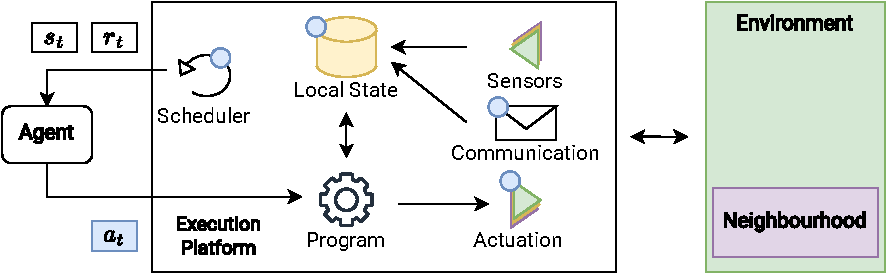
\includegraphics[width=\linewidth]{papers/acsos2022/img//rl-architecture.pdf}
    \caption[Description of the general scheme of \ac{RL} applied to the execution platform.]{Description of the general scheme of \ac{RL} applied to the execution platform. 
    %
    The agent receives the state and reward from the platform and produces an action that can affect one of the platform aspects (blue circles).}
    \label{acsos2022:fig:rl-and-ac}
\end{figure}
In the \ac{AC} framework, 
 we can assume \emph{homogenous} collective behaviours---
 i.e., agents which participate in the aggregate system should execute the same program. 
 In terms of the \ac{RL} process, this means that we could find a single policy for the entire system even if we are in multi-agent settings.%----as pointed out in~\Cref{chap:learning:roadmap}
Specifically, we aim at using a global $Q$-table during the learning time, 
 by which each node uses and refines it with the local experience.
This means that each node, after collecting the typical ($s_t, a_t, r_{t+1}$) trajectory,
 performs the Q-learning update on the shared table.
%
 This way, the $Q$-table encapsulates the knowledge of the whole aggregate behaviour.
%
At the end of the learning phase then, 
 the final $Q$-table is conceptually assigned to the whole system, by sharing the $Q$-table with all the agents.
%
 The nodes consequently follow a greedy policy over that table, 
 which is a typical approach used in \emph{swarm}-like system~\cite{DBLP:journals/jmlr/HuttenrauchSN19, DBLP:conf/atal/SosicKZK17}.
%
In doing so, the policy works for small networks as well as large networks  (i.e, scales with the agent's population size).

%
The agent, however, could \emph{inspect} the learning and evaluation process. 
 Therefore, the agent state should depend on locally produced export and output, 
 and the messages received from the neighbours.
%
The actions chosen by the agents only indirectly influence the local program output: 
 this is done by producing side-effects at the infrastructural level---e.g., 
 dropping obsolete messages from neighbours, 
 or waking up more frequently to more quickly 
 react to locally perceived changes.
%
The actions can also influence the neighbourhood state, e.g., by sending a special message to force neighbours to wake up.
%
This work considers a \emph{local} reward function, that should be crafted in a way that brings about the collective goal through emergence. 
%
However, the reward definition is \revision{specific to the \emph{non-functional requirement} that is being considered; in other cases, there might be the need to design more complex reward functions,}  
such as global functions (i.e., the reward signal is received after collective actions) or neighbourhood-level functions (i.e., the signal is received after a neighbourhood-level action).
\revision{Nevertheless, for the requirement taken into account (e.g., energy efficiency---see next subsection), 
 the reward function can be reused across several collective program specifications,
 since it does not depend on the application logic.
}

\subsection{\Acl{RL} to Reduce Energy Consumption}\label{acsos2022:acrl-energy-goal}
Among the non-functional goals that \ac{RL} could face, 
 this study %analyses the application of Distributed Q-Learning 
 focusses on reducing the \emph{energy consumption} of aggregate computations,
 by altering the local agent \emph{scheduling policy} (As pointed out in \Cref{acsos2022:s:discussion:ac}).
%
\revision{Our goal is to reduce the number of computation rounds and hence the energy needed to achieve certain results in a certain time amount or, dually, 
 to reduce the amount of time to achieve certain results
 for a given amount of energy.}
%
\revision{Similar ideas have already been considered} in related works about Wireless sensor network scheduling.
In~\cite{DBLP:journals/automatica/IwakiWWSJ21,DBLP:journals/ijcnds/MihaylovBTN12} the system learns 
when a node should wake up in order to reduce conflicting messages 
(and therefore to reduce the power consumption). 
However, our work is quite different from the previous. 
We aim to leverage learning to improve a \emph{general} collective computation 
expressed in \ac{AC}-like execution model (i.e, asynchronous and continuous evaluation of \revision{rounds} brings to collective specifications).

In particular, the algorithm should learn how to reduce the round frequency in stable conditions. 
 To this aim, the program should be self-stabilising~\cite{DBLP:journals/tomacs/ViroliABDP18}, 
 i.e., it should reach a well-defined eventual fix-point field result, once input fields cease to change.
\revision{Note that, by reducing the round frequency, 
 we reduce both the total amount of program evaluation \emph{and} 
 the message exchange between neighbours 
 (which typically involves non-negligible power consumption).}

\revision{Even if we consider the whole aggregate computing context as a state, 
 in this work the agent observation space is based on the local output produced by an aggregate program evaluation.} 
 Following the self-stabilisation assumptions, an agent state encodes the variation of the output history, \revision{thus we constrain the output to be a numeric value}.
 At each time step $t$, it is computed the local output $o_t$ and $\delta_t$, which consists of three possible values, \texttt{Stable} ($o_t = o_{t-1}$), \texttt{Rising} ($o_t > o_{t-1}$), and \texttt{Decreasing} ($o_ t < o_{t-1}$).
Also, in order to consider the evolution of $\delta$, each agent stacks the last $w$ values of $\delta$ in its state: $s_t =(\delta_t, \delta_{t-1}, \dots, \delta_{t-w})$.

The actions point out when the agent should fire the next aggregate program evaluation, following a typical wake-up scheduling.
%
We consider a discrete action set, e.g., based on possible energy consumption profiles.
% 
Each action contains the delta time at which the next round should be triggered. 

Finally, the reward function is devised by only observing the local state of the \ac{AC} execution platform, aiming to reduce the overall consumption by emergence.
%
%This way, it is possible to use online learning, without the need for simulations.
The reward signal should consider two aspects: \begin{itemize}
    \item the overall low-power consumption;
    \item the time needed to reach a stable condition.
\end{itemize} 
In doing this, the signal weighs these two contributions using an additional parameter $\theta$.
 When the output history contains a $\delta \neq \text{\texttt{Stable}}$, the reward function is evaluated as:
\begin{equation}
r_t = - \theta * \Delta / T
\end{equation}
$T$ is defined by the action with the highest next wake up value.
%
This gives a negative reward if the node stays in a non-stable condition for a long time (i.e., when $\Delta = T$).
Otherwise, the reward function is evaluated as:
\begin{equation}
r_t = (1 - \theta) * (1 - \Delta / T)
\end{equation}
That is the inverse of the case of non-stable conditions. 
 Thus, this reduces the consumption as much as possible, so the reward is maximized when $\Delta = T$.

Notice that these settings do not depend on a particular aggregate program, 
 but they can be used in any program with continuous output and an eventually stable field. 
%
Besides, thanks to the local reward function, 
 this learning setting could be also employed for online learning.
\revision{However, we would highlight that in this case, 
 we exploited offline learning. 
 In this way, we could consider the cost of \ac{rl} at runtime negligible concerning power consumption.}

\newcommand{\rlsol}{{\sc{}Rl}}
\newcommand{\periodicsol}{{\sc{}Periodic}}
\newcommand{\adhocsol}{{\sc{}Ad-hoc}}
\newcommand{\swapscen}{{\sc{}Swap}}
\newcommand{\multiswap}{{\sc{}MultiSwap}}
\section{Evaluation}\label{acsos2022:sec:evaluation}


Our \ac{RL} approach combined with \ac{AC} is evaluated through a set of simulated experiments, 
 verifying that an aggregate system eventually learns an improved scheduling policy reducing the overall system consumption.
%
To this purpose, we adopt \scafi{}~\cite{DBLP:conf/isola/CasadeiVAD20}, 
 which bundles, together with the language previously discussed, a simulator to execute aggregate programs.

%
For the sake of reproducibility, the code and the instructions to run simulations and produce the charts are open-sourced and available at a public repository\footnote{\url{https://github.com/cric96/experiment-2022-acsos-round-rl}}.
\begin{table}[t]
    \centering
    \begin{tabular}{|l|l|l|}
    \hline
    Parameter & Description & Values                 \\ \hline
    $\epsilon_0$ & $\epsilon$ at the beginning of simulations & {[}0.1, 0.4{]}        \\ \hline
    $\gamma$  & Discount factor for Q update & {[}0.99, 0.95{]}   \\ \hline
    $\alpha$ & Learning rate for Q update & {[} 0.1, 0.4 {]}                    \\ \hline
    $w$     & State window stack size  & {[}2, 5, 7{]}          \\ \hline
    $\theta$ & Balance of reactivity vs. consumption & {[}0.975, 0.9, 0.99{]} \\ \hline
    \end{tabular}
    \caption{The parameters used in simulations. A simulation consist in a tuple of ($\epsilon_0$, $\gamma$, $\alpha$, $w$, $\theta$).}
    \label{acsos2022:tab:parameters}
\end{table}
\subsection{Simulation Setup}\label{acsos2022:s:simulation-setup}
In the experimental setup, we configure the network to consist of a 100x100 meter grid populated with $N=100$ nodes. 
 Each simulation episode is designed to last for 80 seconds of simulated time. 
 For the training phase, we conduct $L=1000$ episodes using an $\epsilon$-greedy policy. 
 The value of $\epsilon$ is dynamically adjusted in each episode $k$ according to the formula:

\begin{equation}
\epsilon_k = \epsilon_0 - (\epsilon_0 / L \times k)
\end{equation}

Here, $\epsilon_0$ serves as the initial value of $\epsilon$. 
 This decay mechanism is implemented to strike an effective balance between exploitation and exploration as the training progresses.

In terms of learning, 
 a single global Q-table is maintained, 
 which each agent updates using local trajectory tuples of the form ($s_t, a_t, r_{t+1}$). 
 Following the training phase, we evaluate the system's performance over the final $T=50$ episodes, 
 employing a greedy policy for this assessment. 
 At this stage, each agent operates with a localized copy of the Q-table, reflecting the state of the system post-training.

The nodes in the grid have the option of executing four distinct actions, corresponding to different next-wake uptimes: 
 100ms, 200ms, 500ms, and 1s. 
 The focus of the training will be on optimizing scheduling policies for two specific programs, 
 referred to as the gradient-cast (G) and the converge-cast (C) building blocks, which are detailed in \Cref{part:background}.

To explore the impact of dynamic changes on the system, 
 we introduce variability in the set of source nodes. 
 When the source set changes, the computational field must recalibrate to a new stable state. 
 Slow response from nodes can significantly extend the convergence time. 
 In scenarios with minor changes, 
 learning algorithms could favor solutions where nodes opt for the longest next wake-up time, thereby reducing responsiveness.

 To induce this variability, 
 we design two specific scenarios. 
 In the first scenario, referred to as \swapscen{}, a single source node is initially placed at the grid's leftmost corner. At time 40, the rightmost node becomes the new source, causing a ripple effect in the system that is eventually stabilized by the aggregate computation.
 
The second scenario, termed \multiswap{}, 
 starts with a central node as the single source. 
 At time 30, four nodes at the grid corners become new sources. 
 At time 60, these corner nodes revert to being non-source nodes.
 
To assess the performance of our RL-based solution (\rlsol{}), 
 we conduct simulations for each parameter set as shown in \Cref{acsos2022:tab:parameters}. 
 We compare \rlsol{} against two alternatives: a fixed-rate scheduling approach (\periodicsol{}) with the minimum wake-up time of 100ms, and a power-minimizing heuristic (\adhocsol{}).
 
Specifically, in \adhocsol{}, nodes adjust their next wake-up time based on output changes. 
 If the output differs from the previous step, 
 they double the next wake-up time, up to a maximum limit. Otherwise, they keep it at the minimum action set value of 100ms.
 
We examine how different parameters influence learning dynamics and quantify the solution error using mean squared error (MRSE) between \periodicsol{} and \rlsol{} as follows:
 
 \begin{equation}
     MRSE_t = \sum_{i=0}^{N} (\text{output}_t(i)^{\text{Periodic}} - \text{output}_t(i)^{\text{RL}})
 \end{equation}
 
 In the above equation, $t$ is the time step at which the error is evaluated, and $i$ indexes individual nodes. 
  We also count the total number of computation rounds (or ``ticks'') across the entire system:
 
 \begin{equation}
     \text{TotalTicks}_t = \sum_{i=0}^{N} (\text{rounds}(i))
 \end{equation}
 
 Here, \texttt{rounds} is a local function that tallies how many times a node has executed the aggregate program. 
  Another metric we consider is the rate of ticks per second:
 
 \begin{equation}
     \text{TicksPerSecond}_t = \text{TotalTicks}_t - \text{TotalTicks}_{t-1}
 \end{equation}
 
For a direct comparison between \rlsol{} and \adhocsol{}, 
 we calculate two additional metrics: 
 the \emph{error percentage} and the \emph{energy saving percentage}. 
% 
The error percentage indicates how much the computational field of \rlsol{} diverges from that of \periodicsol{}. 
 The aim is to minimize this value. 
 The energy saving percentage is calculated as:
 \begin{equation}
     \text{EnergySaving}_t = \frac{\text{TotalTicks}^{\text{Periodic}}_t - \text{TotalTicks}_t}{\text{TotalTicks}^{\text{Periodic}}_t}
 \end{equation}
 
This metric is intended to be maximized, 
 as a higher value indicates more significant power savings.
\subsection{Discussion and Results}\label{acsos2022:s:discussion:ac}
\begin{figure}
    \centering
    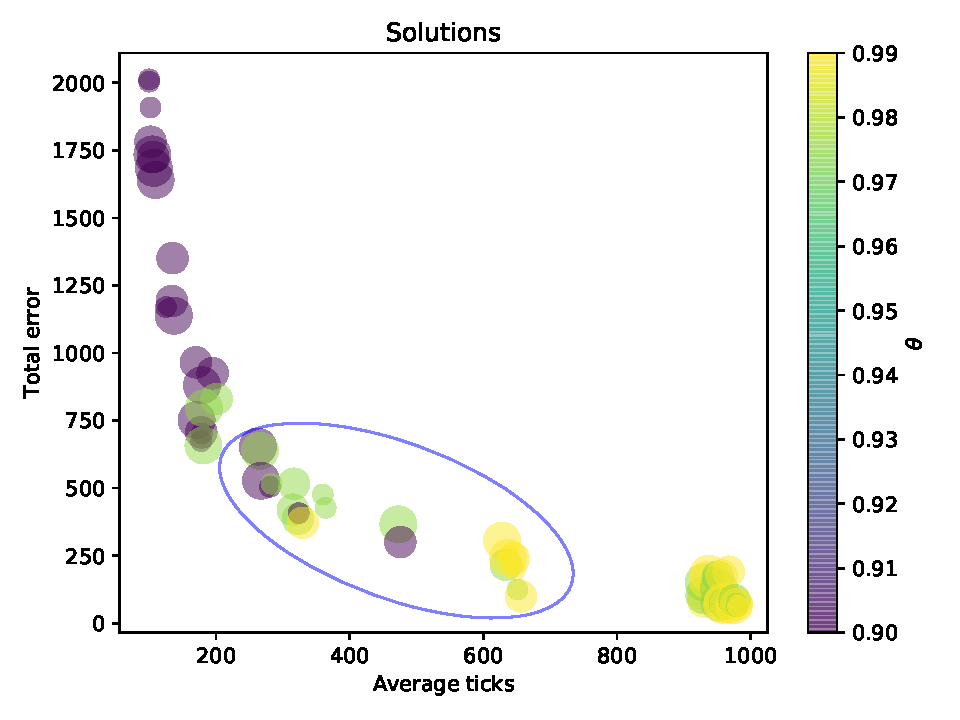
\includegraphics[width=0.5\linewidth]{papers/acsos2022/img//solution-g.pdf}
    \caption[Pareto front varying the $w$ parameter in the scheduling scenario]{The distribution of the solutions after the training phases in \swapscen{} scenario. 
        Each point consists of one of the configurations expressed in \Cref{acsos2022:tab:parameters}.
        The colour of nodes shows the $\theta$ parameter. 
        The size of nodes represents the $w$ value (the smaller the node the smaller the $w$). 
        The solutions of interest are located in the blue ellipse.
        Similar results are achieved with C and in the \multiswap{} scenario. 
    }
    \label{acsos2022:fig:solutions}
\end{figure}
\begin{figure}
    \centering
    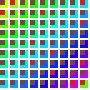
\includegraphics[width=0.2\linewidth]{papers/acsos2022/img//start.png}
    \,
    
\includegraphics[width=0.1\linewidth]{papers/acsos2022/img//arrow.png}
    \,
    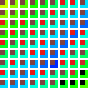
\includegraphics[width=0.2\linewidth]{papers/acsos2022/img//middle.png}
    \,
    
\includegraphics[width=0.1\linewidth]{papers/acsos2022/img//arrow.png}
    \,
    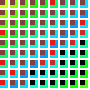
\includegraphics[width=0.2\linewidth]{papers/acsos2022/img//end.png}
    \caption[Scheduling dynamics after the learning phase]{The slow-down behaviour of the policy learnt in \swapscen{} scenario.
    The colours of the small squares denote the node frequencies 
    (the redder, the higher the frequency).
    The colours of the large squares denote the output 
    (the greener, the closest the nodes to the sources).
    In the leftmost figure, a new source appears in the bottom right corner. 
    The signal propagation produces a frequency drop on the node that evaluates the new value 
    (the black node grows toward the gradient direction).
    }\label{acsos2022:fig:simulation-evolution}
\end{figure}

\begin{figure*}
    \centering
    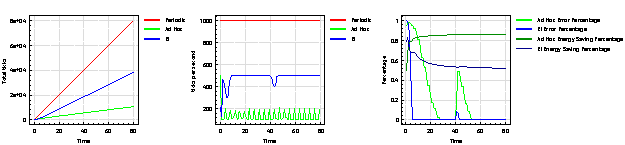
\includegraphics[width=\textwidth]{papers/acsos2022/img//image-rl-500-plain.pdf}
    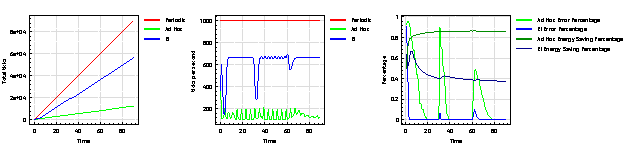
\includegraphics[width=\textwidth]{papers/acsos2022/img//image-rl-500-multi.pdf}
    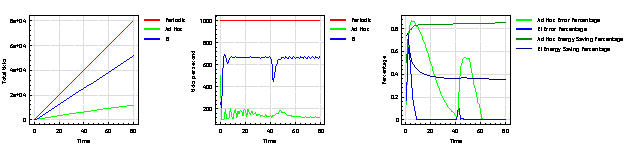
\includegraphics[width=\textwidth]{papers/acsos2022/img//image-rl-500-c.pdf}
    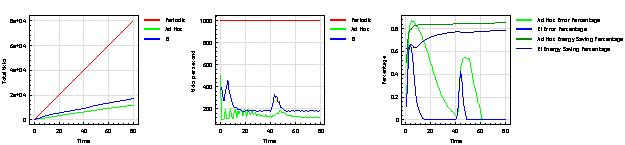
\includegraphics[width=\textwidth]{papers/acsos2022/img//image-rl-500-c-power.pdf}
    \caption[Simulation results of Q-learning applied to schedule aggregate computations]{Simulation results. %Simulation performance encountered using \ac{RL} to manage round firing. 
    % 
    The leftmost chart shows the total ticks as time passes ($ticks$), 
    the chart in the middle shows the ticks per second, and the rightmost chart shows the error and consumption measures. 
    %
    The first line shows the best performance of the gradient-case program in the simplest scenario (i.e., \swapscen{}). 
    %
    The second line evaluates the performance of the gradient in the \multiswap{} scenario.
    %
    Finally, the last two lines show how RL manages the C block, with different $\theta$ values. 
    The overall power-saving using our approach is between 60$\%$ to 40$\%$ with respect to the \periodicsol{} program evaluation.}
    \label{acsos2022:fig:simulation-results}
\end{figure*}

\begin{figure*}
    \centering
    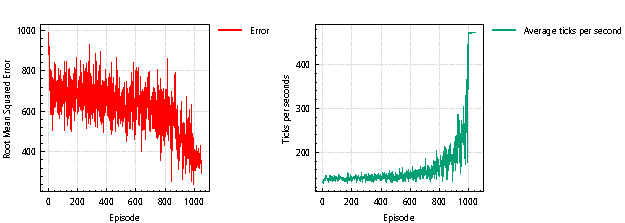
\includegraphics[width=\textwidth]{papers/acsos2022/img//error-and-ticks.pdf}
    \caption{Shows the average error and the average ticks during the learning episodes of \swapscen{} scenario. }
    \label{acsos2022:fig:training-performance}
 \end{figure*}
 \begin{figure}
    \centering
    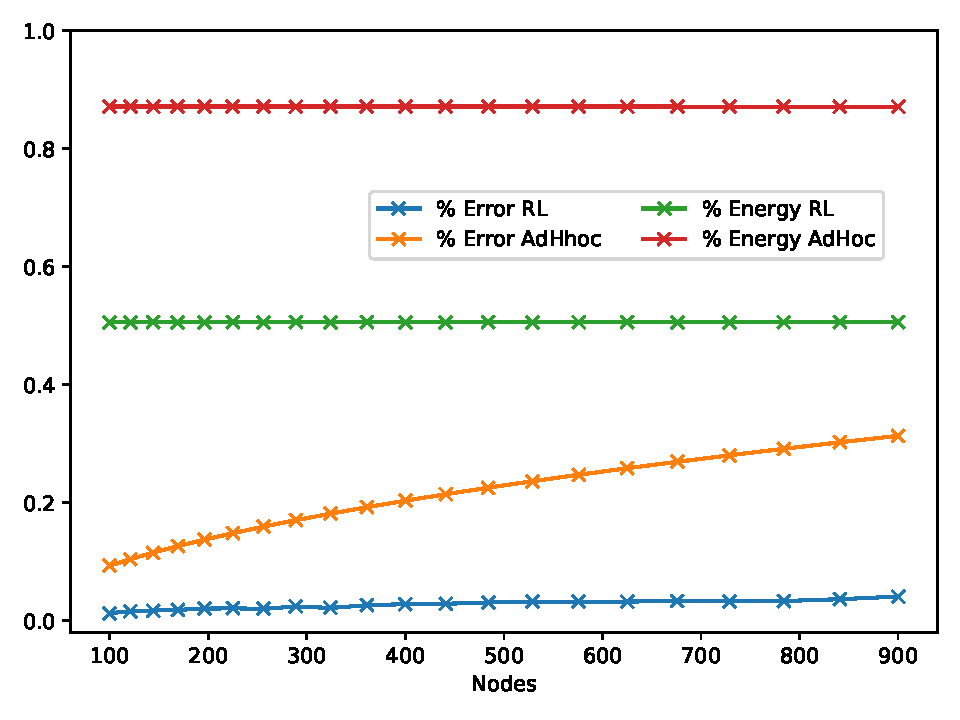
\includegraphics[width=0.8\linewidth]{papers/acsos2022/img//plain-gradient.pdf}
    \caption[Error and energy saving percentage (see \Cref{acsos2022:s:simulation-setup}) as nodes vary.]{\revision{Error and energy saving percentage (see \Cref{acsos2022:s:simulation-setup}) as nodes vary. 
    We use the best policy found in the \swapscen{} scenario as a reference, checking how the error and energy saving change. }}
    \label{acsos2022:fig:check-scale}
 \end{figure}
The simulations demonstrate 
 that the learning algorithm produces different policies. 
 Particularly, observing the \Cref{acsos2022:fig:solutions} we could recognize three macro-behaviours:
\begin{itemize}
    \item the system tends to reduce the power consumption as much as possible, 
     leading to high error and non-reactive policy. 
     It happens mainly with a low value of $\theta$ since the smaller it is 
     the greater the reward for reducing consumption tends to be.
    \item When the simulation runs with a high $\theta$ value, 
    the policies remain with a high power profile to increment 
    as much as possible the reactivity to the environment changes. 
    %
    \item The system tries to balance power efficiency and reactivity, 
    which is our intended goal. 
    It is typically achieved with a value in the middle of the two, 
    but also other parameters influence the training results.
\end{itemize}

This section discusses the results of 
 those simulations that have a high power-saving percentage
 and a low error in each scenario/program
 since the others do not have any particular point of interest. 
%
\Cref{acsos2022:fig:simulation-results} shows the charts of the simulation results.
%
In each scenario, the algorithm successfully 
 reduces the power consumption percentage of the system, 
 maintaining a low percentage of the output error. 
%
 The best performances are typically reached with the highest value of $\theta$, $\gamma$, and $w$.
%
Indeed, the first value guides the learning process 
 to reduce the period in which the node outputs are in an unstable condition. 
%
$\gamma$ tends to reduce the long-term consumption, 
 guiding the node to maximize the overall power.
% 
Finally, with a great value of $w$, 
 agents tend to better understand the output progression and then they better react to local changes. 
 %$\epsilon$ does not seem that alter so much the results in that cases. 

The best results are achieved in the \swapscen{} (\Cref{acsos2022:fig:training-performance})
 scenario and with the gradient program. 
 Here, introducing at most a \revision{10$\%$} of error in the swap moments 
 (i.e., when the new source appears), 
 the learning algorithm reduces the power consumption by nearly 60$\%$.
%
Particularly, the consumption is near to our \adhocsol{} solution, 
 but with a remarkably reduced error. 
%
Interestingly, at the swap time, the round frequency drops until a peak and then soars (\Cref{acsos2022:fig:simulation-evolution}).
This behaviour may appear counter-intuitive.
 At a first glance, indeed, we expect that the nodes tend to maintain a low-cost power consumption, 
 and then when changes in the environment happen, 
 the nodes start to increase the frequency to react quickly against them.
%
However, if the nodes sleep, they cannot intercept new events. 
 For this reason, the agents tend to maintain a high power 
 consumption to identify changes and then they could enter power-saving settings.%

In the \multiswap{} scenario, 
 the algorithm reaches a good performance with a very low error, 
 but with slightly higher power consumption (600 ticks on average versus 500 of the \swapscen{} scenario). 
%
This happens since we gave more importance to the convergence time 
 (with $\theta = 0.99$) and therefore the algorithm tended 
 to prefer solutions with low error. % (i.e, slow convergence time).
%
Nevertheless, even if it has higher consumption, 
 it reaches a similar performance of \periodicsol{} but with half of the ticks.
%

The same \ac{RL} settings could be used even with different programs. 
%
Indeed, the system learns how to reduce consumption also when it is used with block C.
% 
Interestingly, $\theta$ could be used to decide the trade-off 
 between power consumption and reactivity: 
 the program with $\theta=0.9$ (fourth line \Cref{acsos2022:fig:simulation-results}) 
 has a low error but a limited reduction in the power consumption ($\sim$ 40 $\%$); 
 instead, the program with $\theta=0.975$ has an increased convergence 
 time in the swap moments but the overall consumption is reduced by a factor of 70.
 %
%Thus, given some energy constraints, 
% the designer could tune the system consumption by only changing $\theta$.

\revision{
Lastly, we want to recall that \ac{AC} programs are scale-free regarding the number of nodes, 
 since they leverage self-organization to reach a collective structure. 
Therefore, even the learnt policy should not depend on the agents in the system. 
To verify this consideration, we use the same policy found with 
 100 nodes in several other deployments (from 100 nodes to 900). 
 Particularly, in \Cref{acsos2022:fig:check-scale}, the power consumption reduction 
  remains stable as the nodes vary. 
  Moreover, the error is constant too. 
There were some oscillations but the error remains negligible even 
  if the size has 10 times the nodes of the training configuration. 
Differently, the heuristic worsens by a factor of three.}
 \revision{
\subsection{On practical applicability}\label{acsos2022:s:reality-check}
We test our algorithm in simulated scenarios, 
 but it can simply be adapted in a real system, which mainly means:
\begin{enumerate}
    \item define the training phase (offline/online);
    \item integrate the \ac{RL} agent inference to the aggregate middleware% that observes the output and decides when the next tick and when the system will evaluate the program.
\end{enumerate}
For 1) if the learning is performed online, 
 it should be also taken into account the cost of the central server 
 that performs the learning and the communication among the nodes---
 or any technique that allows a global Q table to be maintained and consistently updated 
 (e.g., via gossip algorithm). 
Obviously, in the case of very dense and large-scale networks that is significant. 
 Whereas if simulations are used, the cost of learning is negligible. 
 Currently, our focus has been on the second case---implementing true distributed 
 online learning, a more detailed evaluation is needed to understand the 
 cost of maintaining a central and updated Q table.
%
For 2) on the other hand, there are several aspects to consider. 
 In fact, \ac{AC} can adapt to different computing platforms and communication protocols, 
 as it adopts a fluid approach---see work on pulverization~\cite{DBLP:journals/fi/CasadeiPPVW20}.
Thus, although AC typically does not care about the underlying platform, 
 since our work is heavily dependent on the execution model instead, 
 we have to be sure that this is closer to reality. 
%
Practically, we have to check i) the communication model and ii) the scheduling platform. 
 For ii), the devices should be able to change the energy-saving model 
 at runtime to support our \ac{AC} solution---that is already possible 
 in various embedded systems such as ESP-32.
Regarding communication instead, 
 it could be that some scheduling policies that rely on a communication protocol 
 do not work for another protocol 
 (e.g., a policy trained with wired TCP, does not work well with wireless UDP due to packet collisions, message flooding, etc). 
 Therefore, in the case of simulation, we should have a communication model as detailed as possible 
 to be sure that the policy works in the selected platform too. 
%Finally, this study needs to do a precise reality check against different types of 
% deployment, to understand how this is effective in different types of systems.
 }
\section{Final Remarks}\label{acsos2022:sec:conclusion}

This chapter explores the combination of in combining \ac{RL} with \ac{AC} 
 to optimize non-functional aspects of collective computations such as power consumption, 
 energy bandwidth, and reactivity (in terms of convergence time) as highlighted by 
 the research roadmap. 
%
In particular, this work leverages Q-Learning 
 to reduce the cost of executing \ac{AC} programs 
 in different synthetic scenarios.
%
The contribution \revision{can be framed within a larger} vision in which 
 the designer could mainly focus on functionality and key non-functional aspects (e.g., resiliency)
 at design time, while the platform \revision{is programmed to or instructed to learn} how 
 to optimize less critical but still highly desired non-functional aspects\revision{---acting upon scheduling or deployment~\cite{DBLP:journals/fi/CasadeiPPVW20}}. % by exploiting simulations.

%\balance
%\printbibliography

